\documentclass[11pt]{report}

% ============================================================
% PACKAGES
% ============================================================

\usepackage{amsmath}                            % Mathématiques
\usepackage{amssymb}                            % Symboles mathématiques
\usepackage{array}                              % Tableaux
\usepackage[french]{babel}                      % Langue française
\usepackage{booktabs}                           % Tableaux propres
\usepackage{enumitem}                           % Listes personnalisées
\usepackage{fancybox}                           % Encadrés
\usepackage{fancyhdr}                           % En-têtes et pieds de page
\usepackage{float}                              % Placement des figures
\usepackage[a4paper, margin=2.5cm]{geometry}    % Marges
\usepackage{graphicx}                           % Images
\usepackage{hyperref}                           % Liens
\usepackage{indentfirst}                        % Indentation du premier paragraphe
\usepackage{makecell}                           % Cellules de tableau
\usepackage[protrusion=true, expansion=false]{microtype}                        % Typographie
\usepackage{pdfpages}                           % Inclusion de PDF
\usepackage{setspace}                           % Interligne
\usepackage{siunitx}                            % Unités
\usepackage{soul}                               % Surlignage
\usepackage{tocloft}                            % Table des matières
\usepackage[T1]{fontenc}
\usepackage[utf8]{inputenc}
\usepackage[most]{tcolorbox}
\newtcbtheorem[number within=chapter]{definition}{Définition}%
{colback=gray!5,
 colframe=black!60,
 fonttitle=\bfseries,
 coltitle=black,
 sharp corners,
 boxrule=0.5pt,
 breakable}{def}

% ============================================================
% CONFIGURATION GÉNÉRALE
% ============================================================

\singlespacing
\setlength{\parskip}{0.5em}

\pagestyle{fancy}
\fancyhf{}
\fancyfoot[C]{\thepage}

\renewcommand{\headrulewidth}{0pt}
\renewcommand{\footrulewidth}{0pt}
\renewcommand{\chaptername}{}

\hypersetup{
	colorlinks=true,
	linkcolor=black,
	urlcolor=blue,
	citecolor=black
}

% ============================================================
% DÉBUT DU DOCUMENT
% ============================================================

\begin{document}

% ============================================================
% PAGE DE GARDE
% ============================================================

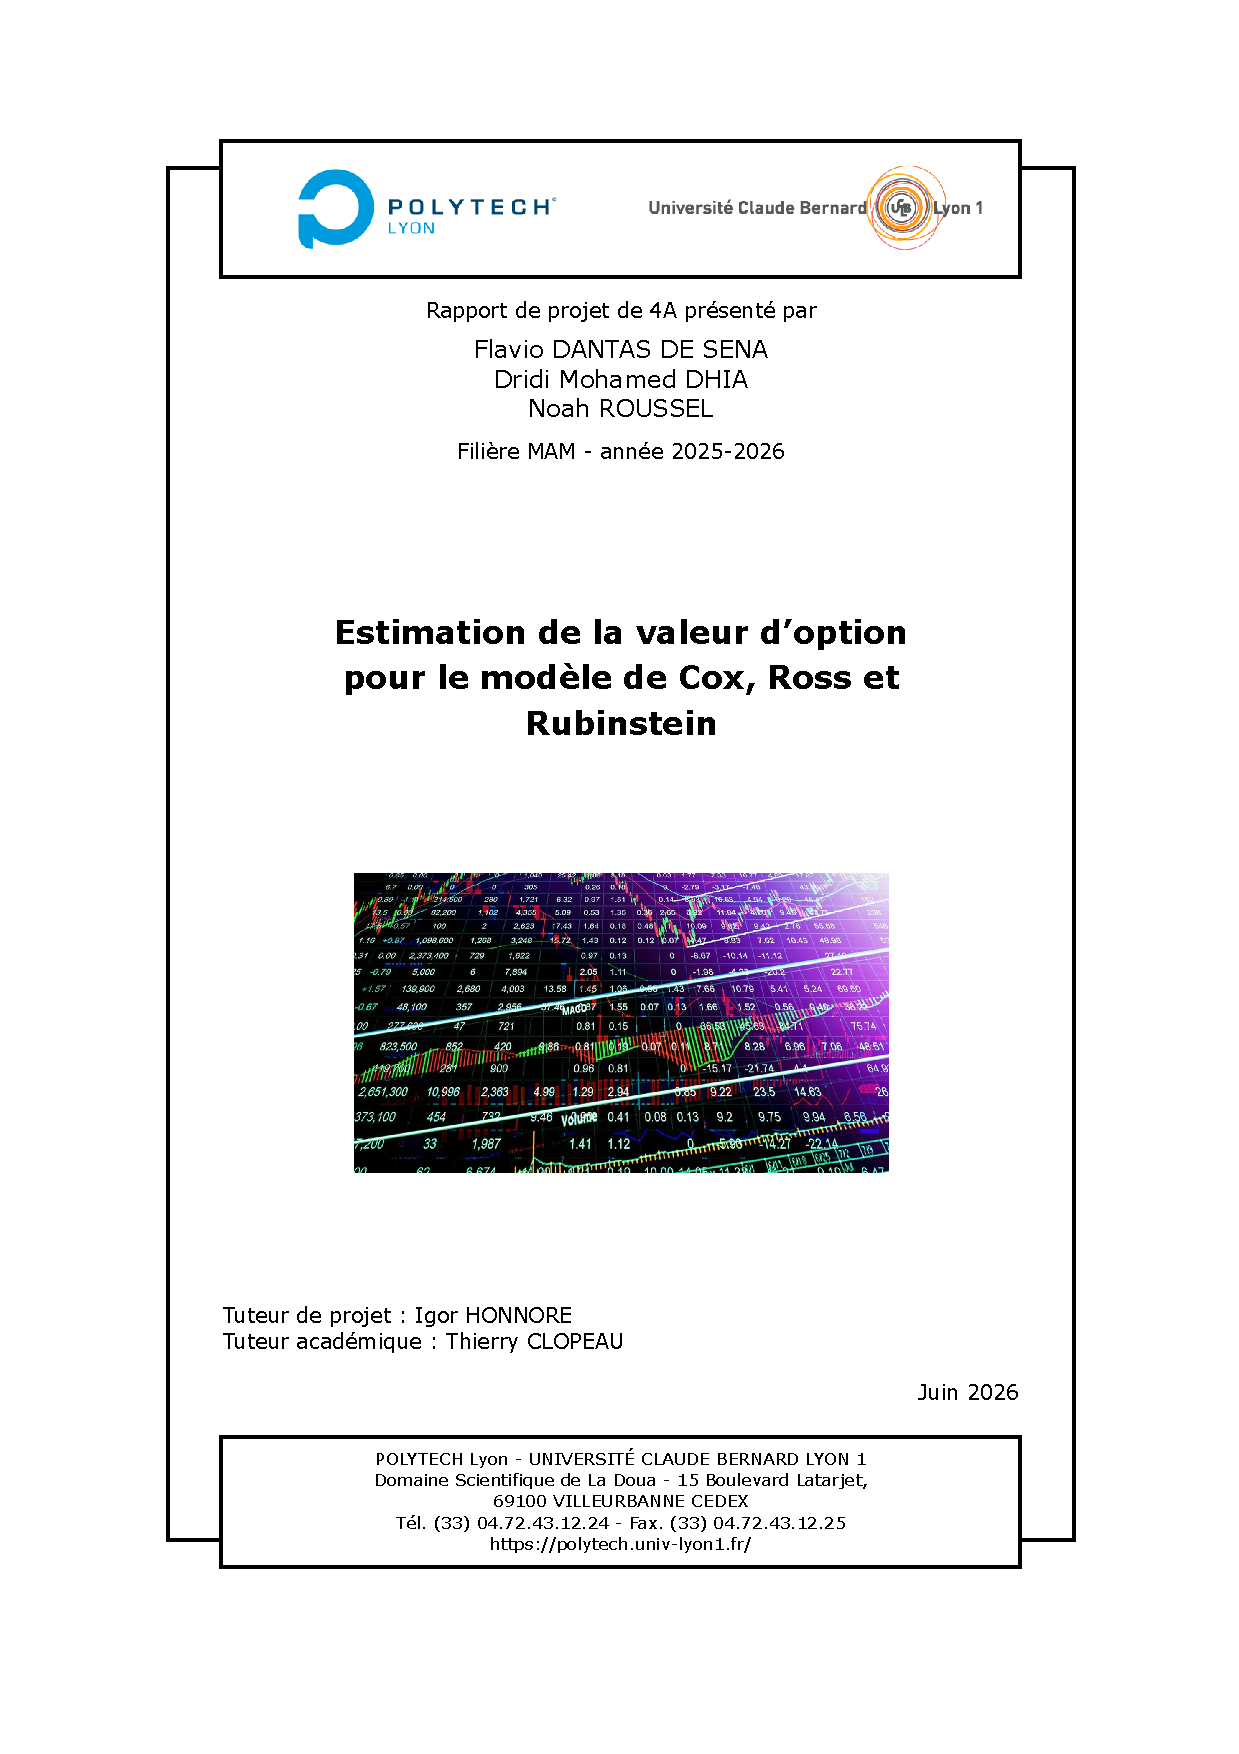
\includepdf[pages=-]{appendix/titlepage.pdf}

% ============================================================
% REMERCIEMENTS
% ============================================================

\chapter*{Remerciements}
\thispagestyle{empty}

% Texte à rédiger.

\newpage

% ============================================================
% RÉSUMÉ
% ============================================================

\chapter*{Résumé}
\addcontentsline{toc}{chapter}{Résumé}

Ce rapport porte sur la valorisation d'options financières à l'aide du modèle binomial de Cox-Ross-Rubinstein. Ce modèle permet de représenter l'évolution possible du prix d'un actif sous-jacent à l'aide d'un arbre binomial, dans lequel le prix peut augmenter ou diminuer à chaque étape.

Après avoir présenté les notions fondamentales liées aux options financières, le rapport introduit le fonctionnement du modèle CRR et les paramètres nécessaires à son application. Une attention particulière est portée à la calibration de ces paramètres à partir de données de marché, notamment à travers le calcul des rendements logarithmiques, l'estimation de la volatilité historique et le choix du taux sans risque.

L'étude est appliquée à différents sous-jacents, dont le CAC 40 et le Brent, afin d'observer le comportement du modèle dans plusieurs contextes de marché. Le modèle est ensuite implémenté informatiquement pour calculer le prix d'options européennes et américaines, puis analyser l'influence des principaux paramètres sur les résultats obtenus.

Ce travail met en évidence l'intérêt du modèle CRR comme outil de valorisation simple, progressif et interprétable, tout en soulignant ses limites, notamment liées aux hypothèses de volatilité constante, de taux sans risque constant et à la sensibilité de la calibration aux données historiques utilisées.


\vspace{1em}

\textbf{Mots-clés :} option financière, modèle binomial, Cox-Ross-Rubinstein, call, put, volatilité, arbre binomial, probabilité risque-neutre, calibration, backtest.

\newpage

% ============================================================
% ABSTRACT
% ============================================================

\chapter*{Abstract}
\addcontentsline{toc}{chapter}{Abstract}

This report focuses on the valuation of financial options using the Cox-Ross-Rubinstein binomial model. This model represents the possible evolution of an underlying asset price through a binomial tree, where the price can either increase or decrease at each time step.

After introducing the main concepts related to financial options, the report presents the CRR model and the parameters required for its implementation. Particular attention is given to the calibration of these parameters from market data, through the computation of logarithmic returns, the estimation of historical volatility and the choice of a risk-free rate.

The study is applied to different underlying assets, including the CAC 40 and Brent, in order to observe the behaviour of the model in several market contexts. The model is then implemented computationally to price European and American options and to analyse the influence of the main parameters on the results obtained.

This work highlights the interest of the CRR model as a simple, progressive and interpretable valuation method, while also pointing out its limitations, especially the assumptions of constant volatility, constant risk-free rate and the sensitivity of the calibration to the historical data used.



\vspace{1em}

\textbf{Keywords:} financial option, binomial model, Cox-Ross-Rubinstein, call, put, volatility, binomial tree, risk-neutral probability, calibration, backtest.

\newpage

% ============================================================
% TABLE DES MATIÈRES
% ============================================================

\pagenumbering{arabic}

\renewcommand{\contentsname}{Table des matières}
\setlength{\cftbeforechapskip}{0.5em}
\tableofcontents

\newpage

% ============================================================
% ABRÉVIATIONS ET NOTATIONS
% ============================================================

\chapter*{Abréviations et notations}
\addcontentsline{toc}{chapter}{Abréviations et notations}

\section*{Abréviations et acronymes}
\addcontentsline{toc}{section}{Abréviations et acronymes}

\begin{center}
	\begin{minipage}[t]{0.49\textwidth}
		\begin{itemize}[noitemsep]
			\raggedright
			\item CRR : Cox, Ross et Rubinstein
			\item CAC 40 : indice boursier français
			\item MAE : Mean Absolute Error
			\item RMSE : Root Mean Squared Error
		\end{itemize}
	\end{minipage}
	\hfill
	\begin{minipage}[t]{0.49\textwidth}
		\begin{itemize}[noitemsep]
			\raggedright
			\item ATM : At The Money
			\item ITM : In The Money
			\item OTM : Out of The Money
			\item OHLCV : Open, High, Low, Close, Volume
		\end{itemize}
	\end{minipage}
\end{center}

\section*{Notations}
\addcontentsline{toc}{section}{Notations}

\begin{center}
	\begin{minipage}[t]{0.49\textwidth}
		\textbf{Notations financières}
		\begin{itemize}[noitemsep]
			\raggedright
			\item $S_0$ : prix initial du sous-jacent
			\item $S_T$ : prix du sous-jacent à maturité
			\item $K$ : prix d’exercice
			\item $T$ : maturité de l’option
			\item $r$ : taux sans risque
			\item $\sigma$ : volatilité du sous-jacent
		\end{itemize}
	\end{minipage}
	\hfill
	\begin{minipage}[t]{0.49\textwidth}
		\textbf{Notations du modèle CRR}
		\begin{itemize}[noitemsep]
			\raggedright
			\item $N$ : nombre d’étapes de l’arbre
			\item $\Delta t$ : pas de temps
			\item $u$ : facteur de hausse
			\item $d$ : facteur de baisse
			\item $p^*$ : probabilité risque-neutre
			\item $V_{i,j}$ : valeur de l’option au nœud $(i,j)$
		\end{itemize}
	\end{minipage}
\end{center}

\newpage

% ============================================================
% INTRODUCTION
% ============================================================

\chapter*{Introduction}
\addcontentsline{toc}{chapter}{Introduction}

% Introduction à rédiger.

\newpage

% ============================================================
% CHAPITRE 1
% ============================================================

\chapter{Cadre théorique financier}

Ce chapitre présente les concepts fondamentaux nécessaires à la compréhension des options financières et de leur valorisation. Avant d’aborder les modèles numériques utilisés pour calculer le prix d’une option, il est important de définir précisément les notions financières de base telles que l'actif sous-jacent, l'option financière, le prix d'exercice, la maturité, le payoff, l'option européenne et l'option américaine.

L’objectif de ce chapitre est donc de construire progressivement le cadre théorique du rapport. Nous commencerons par présenter la notion d’option financière, puis nous distinguerons les deux grands types d’options classiques dont le call et le put. Nous introduirons ensuite la notion de payoff, qui permet de décrire le gain obtenu à l’échéance d’une option. Enfin, nous présenterons les principales caractéristiques influençant le prix d’une option, comme le prix du sous-jacent, la volatilité, le taux d’intérêt, la maturité et le prix d’exercice.

Ces définitions seront ensuite utilisées dans les chapitres suivants pour mettre en place le modèle binomial de Cox-Ross-Rubinstein et calibrer ses paramètres à partir de données de marché.

\section{Définition d'une option financière}

Les options financières appartiennent à la famille des produits dérivés. Avant de définir précisément une option financière, il est donc nécessaire d'introduire d'abord la notion de produit dérivé, puis celle d'actif sous-jacent.

\begin{definition}{Produit dérivé}{produit-derive}
Un produit dérivé est un instrument financier dont la valeur dépend de l'évolution d'un autre actif, appelé actif sous-jacent.
\end{definition}

\begin{definition}{Actif sous-jacent}{actif-sous-jacent}
Un actif sous-jacent est l'actif financier sur lequel repose un produit dérivé.

Il peut s'agir par exemple :
\begin{itemize}
    \item d'une action ;
    \item d'un indice boursier ;
    \item d'une devise ;
    \item d'une matière première ;
    \item d'une obligation.
\end{itemize}

On note généralement le prix de l'actif sous-jacent à la date $t$ par :
\[
S_t.
\]
\end{definition}

Dans le cadre de ce rapport, l'actif sous-jacent considéré sera principalement une action. L'évolution de son prix au cours du temps jouera un rôle central dans la valorisation de l'option.

Une option financière est un contrat portant sur un actif sous-jacent. Elle donne à son détenteur un droit, mais pas une obligation. Ce droit peut être un droit d'achat ou un droit de vente.

\begin{definition}{Option financière}{option-financiere}
Une option financière est un contrat qui donne à son détenteur le droit, mais non l'obligation, d'acheter ou de vendre un actif sous-jacent à un prix fixé à l'avance, à une date donnée ou pendant une période donnée.
\end{definition}

Le prix fixé à l'avance dans le contrat est appelé prix d'exercice.

\begin{definition}{Prix d'exercice}{prix-exercice}
Le prix d'exercice, noté $K$, est le prix auquel le détenteur de l'option peut acheter ou vendre l'actif sous-jacent si l'option est exercée.
\end{definition}

Une option se distingue donc d'un contrat classique par le fait que son détenteur possède un droit, mais n'est jamais obligé de l'exercer. Cette propriété est essentielle : si l'exercice de l'option est défavorable, le détenteur peut choisir de ne pas exercer son droit.

Le contrat d'option est également associé à une date limite. Cette date est appelée maturité ou échéance.

\begin{definition}{Maturité}{maturite}
La maturité, notée $T$, désigne la date d'échéance du contrat d'option.

À cette date, selon le type d'option considéré, le détenteur peut exercer son droit d'achat ou de vente.
\end{definition}

Une option financière est donc principalement caractérisée par les éléments suivants :
\begin{itemize}
   \item $S_t$, le prix du sous-jacent à la date $t$ ;
   \item $K$, le prix d'exercice ;
   \item $T$, la maturité de l'option.
\end{itemize}

Enfin, pour obtenir ce droit, l'acheteur de l'option doit payer un prix. Ce prix est appelé prime de l'option.

\begin{definition}{Prime d'une option}{prime-option}
La prime d'une option est le prix payé par l'acheteur pour obtenir le droit associé au contrat d'option.

Elle représente également le prix de marché de l'option à la date considérée.
\end{definition}

Dans la suite du rapport, l'objectif sera de comprendre comment déterminer cette prime à l'aide de modèles mathématiques. Pour cela, il faudra d'abord distinguer les deux types fondamentaux d'options : les options d'achat, appelées \textit{calls}, et les options de vente, appelées \textit{puts}.

%%% CALL ET PUT %%%

\section{Call et put}

Les options financières sont des instruments échangés sur les marchés financiers. Avant de distinguer les deux formes principales d'options, il est utile de préciser brièvement ce que l'on entend par marché financier.

\begin{definition}{Marché financier}{marche-financier}
Un marché financier est un lieu, physique ou électronique, sur lequel des agents économiques peuvent acheter et vendre des actifs financiers, comme des actions, des obligations, des devises ou des produits dérivés.
\end{definition}

Dans ce cadre, les options financières permettent aux investisseurs de prendre position sur l'évolution future d'un actif sous-jacent. Une option peut donner un droit d'achat ou un droit de vente sur cet actif. Ces deux cas correspondent respectivement au \textit{call} et au \textit{put}.

\begin{definition}{Option d'achat ou call}{call}
Une option d'achat, appelée \textit{call}, est une option qui donne à son détenteur le droit, mais non l'obligation, d'acheter un actif sous-jacent à un prix fixé à l'avance, appelé prix d'exercice.

On note $K$ le prix d'exercice et $S_T$ le prix du sous-jacent à la maturité $T$. Le call présente un intérêt pour son détenteur lorsque
\[
S_T > K.
\]
Dans cette situation, l'acheteur du call peut acheter l'actif au prix $K$, alors que sa valeur de marché est $S_T$.
\end{definition}

Le call est donc associé à une anticipation de hausse du prix du sous-jacent. Lorsque le prix de marché devient supérieur au prix d'exercice, l'exercice de l'option permet d'acheter l'actif à un prix inférieur à sa valeur observée sur le marché. En revanche, si $S_T \leq K$, l'exercice n'est pas avantageux, car l'actif peut être acheté directement sur le marché à un prix inférieur ou égal à $K$.

\begin{definition}{Option de vente ou put}{put}
Une option de vente, appelée \textit{put}, est une option qui donne à son détenteur le droit, mais non l'obligation, de vendre un actif sous-jacent à un prix fixé à l'avance, appelé prix d'exercice.

On note $K$ le prix d'exercice et $S_T$ le prix du sous-jacent à la maturité $T$. Le put présente un intérêt pour son détenteur lorsque
\[
S_T < K.
\]
Dans cette situation, l'acheteur du put peut vendre l'actif au prix $K$, alors que sa valeur de marché est $S_T$.
\end{definition}

Le put est donc associé à une anticipation de baisse du prix du sous-jacent. Lorsque le prix de marché devient inférieur au prix d'exercice, l'exercice de l'option permet de vendre l'actif à un prix supérieur à sa valeur observée sur le marché. En revanche, si $S_T \geq K$, l'exercice n'est pas avantageux, car l'actif peut être vendu directement sur le marché à un prix supérieur ou égal à $K$.

Ainsi, le call et le put reposent sur deux situations opposées. Le call devient intéressant lorsque le prix du sous-jacent dépasse le prix d'exercice, tandis que le put devient intéressant lorsque le prix du sous-jacent devient inférieur au prix d'exercice. Cette distinction permettra, dans la section suivante, d'introduire la notion de payoff, c'est-à-dire le gain obtenu à la maturité selon l'évolution du prix du sous-jacent.

%%%% PAYOFF %%%%

\section{Payoff}

Après avoir distingué les deux types fondamentaux d'options, le call et le put, il est nécessaire d'introduire la notion de payoff. Cette notion permet de mesurer ce que rapporte une option à sa maturité, avant de prendre en compte le prix payé pour l'acheter.

\begin{definition}{Payoff d'une option}{payoff-option}
Le payoff d'une option désigne le gain obtenu par le détenteur de l'option à la maturité $T$, en fonction du prix final du sous-jacent $S_T$ et du prix d'exercice $K$.

Il ne tient pas compte de la prime payée pour acheter l'option.
\end{definition}

Le payoff dépend donc de la position relative entre le prix du sous-jacent à la maturité, noté $S_T$, et le prix d'exercice, noté $K$. Si l'exercice de l'option est avantageux, le payoff est positif. Dans le cas contraire, le détenteur choisit de ne pas exercer son droit, et le payoff est nul.

Pour une option d'achat, le détenteur exerce son droit seulement lorsque le prix du sous-jacent est supérieur au prix d'exercice. Le payoff d'un call est donc donné par la quantité positive entre $S_T - K$ et $0$.

\begin{definition}{Payoff d'un call}{payoff-call}
Le payoff d'un call à la maturité $T$ est donné par
\[
\Pi_{\text{call}}(S_T) = \max(S_T - K, 0).
\]

Ainsi, si $S_T > K$, le payoff vaut
\[
\Pi_{\text{call}}(S_T) = S_T - K.
\]

Si $S_T \leq K$, le payoff vaut
\[
\Pi_{\text{call}}(S_T) = 0.
\]
\end{definition}

Cette formule traduit directement le fonctionnement économique du call. Lorsque le prix du sous-jacent dépasse le prix d'exercice, l'acheteur peut acheter l'actif à un prix inférieur à sa valeur de marché. L'écart $S_T - K$ représente alors le gain obtenu à l'exercice. Lorsque $S_T \leq K$, l'exercice n'est pas avantageux, et le détenteur laisse l'option expirer.

Pour une option de vente, la situation est inverse. Le détenteur exerce son droit lorsque le prix du sous-jacent est inférieur au prix d'exercice. Le payoff d'un put est donc donné par la quantité positive entre $K - S_T$ et $0$.

\begin{definition}{Payoff d'un put}{payoff-put}
Le payoff d'un put à la maturité $T$ est donné par
\[
\Pi_{\text{put}}(S_T) = \max(K - S_T, 0).
\]

Ainsi, si $S_T < K$, le payoff vaut
\[
\Pi_{\text{put}}(S_T) = K - S_T.
\]

Si $S_T \geq K$, le payoff vaut
\[
\Pi_{\text{put}}(S_T) = 0.
\]
\end{definition}

Cette formule exprime l'intérêt économique du put. Lorsque le prix du sous-jacent devient inférieur au prix d'exercice, l'acheteur du put peut vendre l'actif au prix $K$, alors que sa valeur de marché est plus faible. L'écart $K - S_T$ représente alors le gain obtenu à l'exercice. Lorsque $S_T \geq K$, il n'est pas avantageux d'exercer l'option, et le payoff est nul.

Il est important de distinguer le payoff du profit réel de l'investisseur.

\begin{definition}{Profit d'une option}{profit-option}
Le profit d'une option correspond au payoff diminué de la prime payée pour acheter l'option.

Si la prime est notée $C_0$ pour un call, alors le profit du call est donné par
\[
\Pi_{\text{call}}(S_T) - C_0.
\]

Si la prime est notée $P_0$ pour un put, alors le profit du put est donné par
\[
\Pi_{\text{put}}(S_T) - P_0.
\]
\end{definition}

Le payoff mesure uniquement le gain obtenu à la maturité grâce à l'exercice de l'option. Le profit, lui, prend aussi en compte la prime payée au départ pour acheter cette option.

Cette distinction entre payoff et profit est importante, car elle permet de séparer le gain obtenu à l'exercice de l'option du coût initial payé pour acquérir ce droit. Dans la suite, nous nous intéresserons également au moment auquel ce droit peut être exercé. Cette question conduit à distinguer les options européennes et les options américaines.

\section{Options européennes et américaines}

Après avoir défini le payoff d'une option, il est nécessaire de préciser à quel moment le détenteur peut exercer son droit. En effet, toutes les options ne possèdent pas les mêmes règles d'exercice. On distingue principalement les options européennes et les options américaines.

\begin{definition}{Option européenne}{option-europeenne}
Une option européenne est une option qui ne peut être exercée qu'à sa date de maturité $T$.

Ainsi, le détenteur de l'option prend sa décision uniquement à l'échéance, en comparant le prix du sous-jacent $S_T$ au prix d'exercice $K$.
\end{definition}

Dans le cas d'une option européenne, le détenteur ne peut donc pas exercer son droit avant la date $T$. Même si l'option devient avantageuse avant l'échéance, il doit attendre la maturité pour décider s'il exerce ou non son droit.

Pour un call européen, l'exercice est intéressant à la maturité lorsque
\[
S_T > K.
\]
Pour un put européen, l'exercice est intéressant à la maturité lorsque
\[
S_T < K.
\]

\begin{definition}{Option américaine}{option-americaine}
Une option américaine est une option qui peut être exercée à tout moment entre la date d'achat du contrat et sa maturité $T$.
\end{definition}

Contrairement à l'option européenne, l'option américaine donne donc plus de flexibilité à son détenteur. Celui-ci peut choisir d'exercer son droit avant l'échéance si cela lui semble avantageux. Cette liberté supplémentaire rend généralement la valorisation d'une option américaine plus complexe, car il faut étudier la possibilité d'exercice à chaque date avant la maturité.

On peut résumer la différence principale de la manière suivante. Une option européenne ne peut être exercée qu'à la date finale $T$, tandis qu'une option américaine peut être exercée à n'importe quelle date avant ou à la maturité.

Cette distinction est importante, car le moment d'exercice influence la valeur de l'option. Cependant, le type d'exercice n'est pas le seul élément à prendre en compte. Le prix d'une option dépend également de plusieurs paramètres financiers, comme le prix du sous-jacent, le prix d'exercice, la maturité, la volatilité ou encore le taux d'intérêt. Ces paramètres sont présentés dans la section suivante.
%%% PARAMETRES INFLUENCANT LE PRIX D'UNE OPTION %%%
\section{Paramètres influençant le prix d'une option}

Le prix d'une option, aussi appelé prime, dépend de plusieurs paramètres financiers. Certains ont déjà été introduits précédemment, comme le prix du sous-jacent $S_t$, le prix d'exercice $K$ et la maturité $T$. Ces grandeurs jouent un rôle central dans la valorisation, car elles déterminent les conditions dans lesquelles l'option peut devenir avantageuse pour son détenteur.

Le prix du sous-jacent $S_t$ influence directement la valeur de l'option. Pour un call, une hausse du prix du sous-jacent tend à augmenter la valeur de l'option, car le droit d'acheter l'actif au prix $K$ devient plus intéressant. À l'inverse, pour un put, une baisse du prix du sous-jacent tend à augmenter la valeur de l'option, car le droit de vendre l'actif au prix $K$ devient plus avantageux.

Le prix d'exercice $K$ intervient également dans la valeur de l'option. Pour un call, plus $K$ est faible, plus l'option est favorable à son détenteur. Pour un put, c'est l'inverse : plus $K$ est élevé, plus l'option est intéressante, car elle permet de vendre le sous-jacent à un prix supérieur.

La maturité $T$ joue aussi un rôle important. Plus la durée restante avant l'échéance est longue, plus le prix du sous-jacent a le temps d'évoluer. Une maturité plus longue peut donc augmenter la valeur d'une option, car elle laisse davantage de possibilités pour que l'option devienne favorable.

Un autre paramètre essentiel est la volatilité du sous-jacent. Elle mesure l'intensité des variations du prix de l'actif au cours du temps.

La volatilité est généralement estimée à partir des rendements du sous-jacent. Il est donc nécessaire de préciser ce que l'on appelle un rendement.

\begin{definition}{Rendement d'un actif financier}{rendement}
Le rendement d'un actif financier mesure la variation relative de son prix entre deux dates.

Si $S_{i-1}$ désigne le prix de l'actif à la date $i-1$ et $S_i$ son prix à la date $i$, le rendement simple est défini par
\[
R_i^{\mathrm{simple}} = \frac{S_i - S_{i-1}}{S_{i-1}}.
\]

On peut également utiliser le rendement logarithmique, défini par
\[
R_i = \ln\left(\frac{S_i}{S_{i-1}}\right).
\]
\end{definition}

Dans la suite du rapport, nous utiliserons principalement les rendements logarithmiques. Ce choix est courant en finance, car ils possèdent des propriétés mathématiques intéressantes, notamment l'additivité sur plusieurs périodes. En effet, pour trois dates successives $0$, $1$ et $2$, on a
\[
\ln\left(\frac{S_2}{S_0}\right)
=
\ln\left(\frac{S_1}{S_0}\right)
+
\ln\left(\frac{S_2}{S_1}\right).
\]

Cette propriété facilite l'étude des séries financières et l'estimation de la volatilité à partir de données historiques.
\begin{definition}{Volatilité}{volatilite}
La volatilité mesure l'ampleur des fluctuations du prix d'un actif financier au cours du temps. Dans le cadre des options, elle est généralement notée $\sigma$.

Si l'on dispose d'une série de rendements $R_1, R_2, \ldots, R_n$, la volatilité historique peut être estimée par l'écart-type des rendements :
\[
\sigma = \sqrt{\frac{1}{n-1}\sum_{i=1}^{n}(R_i-\bar R)^2},
\]
où
\[
\bar R = \frac{1}{n}\sum_{i=1}^{n} R_i
\]
désigne le rendement moyen observé.
\end{definition}

Une volatilité élevée signifie que le prix du sous-jacent peut varier fortement. Cela augmente la probabilité que l'option devienne avantageuse avant ou à la maturité. Ainsi, une hausse de la volatilité tend généralement à augmenter la valeur d'un call comme celle d'un put.

Enfin, le taux d'intérêt sans risque intervient dans les modèles de valorisation, car il permet d'actualiser les valeurs futures.

\begin{definition}{Taux sans risque}{taux-sans-risque}
Le taux sans risque, noté $r_f$, est le taux de rendement théorique d'un placement considéré comme sans risque sur une période donnée.

Il est utilisé pour ramener une valeur future à sa valeur actuelle.
\end{definition}

Le taux sans risque influence donc la valeur actuelle des montants payés ou reçus dans le futur. Dans les modèles de valorisation d'options, il intervient notamment dans l'actualisation des payoffs futurs.

Ainsi, les principaux paramètres utilisés pour valoriser une option sont le prix du sous-jacent $S_t$, le prix d'exercice $K$, la maturité $T$, la volatilité $\sigma$ et le taux sans risque $r_f$. Ces grandeurs seront utilisées dans la suite du rapport pour construire le modèle binomial de Cox-Ross-Rubinstein.
\newpage

% ============================================================
% CHAPITRE 2
% ============================================================

\chapter{Modèle de Cox, Ross et Rubinstein}

Après avoir présenté les notions financières fondamentales liées aux options, nous pouvons maintenant introduire un premier modèle de valorisation. L'objectif est de déterminer, à partir des paramètres du contrat et du marché, une estimation du prix d'une option.

Dans ce chapitre, nous présentons le modèle binomial de Cox, Ross et Rubinstein, souvent appelé modèle CRR. Ce modèle repose sur une représentation discrète de l'évolution du prix du sous-jacent. À chaque période, le prix peut seulement évoluer selon deux possibilités : une hausse ou une baisse. Cette structure permet de construire un arbre de prix, puis de calculer progressivement la valeur de l'option.

\section{Principe général du modèle binomial}

Le modèle de Cox, Ross et Rubinstein propose une méthode de valorisation des options fondée sur une représentation discrète du temps. Au lieu de supposer que le prix du sous-jacent évolue de manière continue, le modèle découpe la durée de vie de l'option en un nombre fini d'étapes.

À chaque étape, le prix du sous-jacent peut évoluer de deux manières. Il peut augmenter selon un facteur de hausse, noté $u$, ou diminuer selon un facteur de baisse, noté $d$.

\begin{definition}{Modèle binomial}{modele-binomial}
Un modèle binomial est un modèle dans lequel, à chaque période, le prix du sous-jacent ne peut prendre que deux évolutions possibles : une hausse ou une baisse.
\end{definition}

Dans le modèle CRR, si le prix du sous-jacent vaut $S$ à une date donnée, alors à la période suivante il peut devenir
\[
Su
\]
en cas de hausse, ou
\[
Sd
\]
en cas de baisse.

On suppose généralement que
\[
u > 1
\qquad \text{et} \qquad
0 < d < 1.
\]

Le facteur $u$ représente donc une évolution positive du prix du sous-jacent, tandis que le facteur $d$ représente une évolution négative. En répétant cette construction sur plusieurs périodes, on obtient un arbre binomial représentant les différentes valeurs possibles du sous-jacent jusqu'à la maturité de l'option.

\begin{definition}{Arbre binomial}{arbre-binomial}
Un arbre binomial est une structure qui représente les différentes évolutions possibles du prix d'un actif lorsque, à chaque étape, ce prix peut soit augmenter, soit diminuer.
\end{definition}

L'intérêt du modèle binomial est qu'il permet de calculer le prix d'une option de manière progressive. On commence par déterminer les valeurs possibles du sous-jacent à la maturité, puis on calcule les payoffs associés. Ensuite, on remonte l'arbre jusqu'à la date initiale afin d'obtenir le prix de l'option aujourd'hui.

Avant de construire cet arbre plus précisément, il est nécessaire de présenter les hypothèses sur lesquelles repose le modèle CRR.

\section{Hypothèses du modèle}

Comme tout modèle financier, le modèle CRR repose sur plusieurs hypothèses simplificatrices. Ces hypothèses permettent d'obtenir un cadre mathématique clair pour valoriser les options, même si elles ne décrivent pas parfaitement la réalité des marchés.

On suppose d'abord que le marché est sans friction. Cela signifie que l'on néglige les coûts de transaction, les taxes et les contraintes liées à l'achat ou à la vente des actifs. Cette hypothèse simplifie les calculs et permet de se concentrer sur la logique de valorisation.

Le taux sans risque, noté $r_f$, est supposé constant pendant toute la durée de vie de l'option. Cette hypothèse permet d'utiliser un même taux pour actualiser les valeurs futures dans l'arbre binomial.

Le modèle suppose aussi que la volatilité du sous-jacent, notée $\sigma$, reste constante sur la période étudiée. Cela signifie que l'intensité des variations du prix du sous-jacent ne change pas au cours du temps.

Enfin, le modèle repose sur l'absence d'opportunité d'arbitrage. Cette hypothèse est fondamentale, car elle garantit la cohérence du prix obtenu.

\begin{definition}{Absence d'opportunité d'arbitrage}{absence-arbitrage}
L'absence d'opportunité d'arbitrage signifie qu'il est impossible de construire une stratégie permettant d'obtenir un gain certain sans risque et sans investissement initial.
\end{definition}

Ces hypothèses permettent de construire un modèle simple et cohérent. Elles fixent le cadre dans lequel le prix du sous-jacent sera représenté de manière discrète.

Il faut maintenant préciser comment la durée de vie de l'option est découpée en plusieurs étapes.

\section{Discrétisation du temps}

Le modèle CRR travaille en temps discret. Cela signifie que la durée de vie de l'option n'est pas considérée comme continue, mais découpée en plusieurs périodes de même longueur.

Si la maturité de l'option est notée $T$ et si l'on choisit de découper cette période en $N$ étapes, alors la durée d'une étape est notée $\Delta t$.

\begin{definition}{Pas de temps}{pas-de-temps}
Le pas de temps, noté $\Delta t$, désigne la durée d'une période élémentaire dans l'arbre binomial.

Il est défini par
\[
\Delta t = \frac{T}{N},
\]
où $T$ est la maturité de l'option et $N$ le nombre d'étapes de l'arbre.
\end{definition}

Ainsi, plus le nombre d'étapes $N$ est grand, plus le pas de temps $\Delta t$ est petit. L'arbre décrit alors l'évolution du sous-jacent de manière plus fine.

À l'étape $i$, le temps correspondant est donné par
\[
t_i = i\Delta t,
\]
avec
\[
i = 0,1,\ldots,N.
\]

L'étape $i=0$ correspond à la date initiale, tandis que l'étape $i=N$ correspond à la maturité de l'option.

Une fois ce découpage temporel défini, on peut construire l'arbre des prix du sous-jacent en associant à chaque étape les mouvements possibles de hausse et de baisse.

\section{Construction de l'arbre des prix}

L'arbre binomial est construit à partir du prix initial du sous-jacent, noté $S_0$. À chaque étape, le prix peut être multiplié par le facteur de hausse $u$ ou par le facteur de baisse $d$.

On repère chaque nœud de l'arbre par deux indices $(i,j)$, où $i$ représente l'étape temporelle et $j$ le nombre de hausses observées depuis la date initiale.

\begin{definition}{Prix au nœud de l'arbre}{prix-noeud}
Dans l'arbre binomial, le prix du sous-jacent au nœud $(i,j)$ est donné par
\[
S_{i,j} = S_0 u^j d^{i-j},
\]
où $i$ désigne l'étape de l'arbre et $j$ le nombre de hausses observées.
\end{definition}

Dans cette formule, le terme $u^j$ correspond aux $j$ hausses successives, tandis que le terme $d^{i-j}$ correspond aux $i-j$ baisses. Ainsi, à une étape donnée $i$, plusieurs valeurs du sous-jacent sont possibles selon le nombre de hausses et de baisses réalisées.

Le choix des facteurs $u$ et $d$ est essentiel dans le modèle CRR. Ils sont définis à partir de la volatilité $\sigma$ et du pas de temps $\Delta t$.

\begin{definition}{Facteur de hausse}{facteur-hausse}
Dans le modèle CRR, le facteur de hausse est noté $u$ et défini par
\[
u = e^{\sigma\sqrt{\Delta t}}.
\]
\end{definition}

Le facteur $u$ mesure l'augmentation possible du prix du sous-jacent pendant une période. Plus la volatilité $\sigma$ est élevée, plus le facteur de hausse est important.

\begin{definition}{Facteur de baisse}{facteur-baisse}
Dans le modèle CRR, le facteur de baisse est noté $d$ et défini par
\[
d = e^{-\sigma\sqrt{\Delta t}}.
\]
\end{definition}

On remarque que
\[
d = \frac{1}{u}.
\]

Cette relation permet d'obtenir un arbre recombiné.

L'arbre permet donc de représenter les différents prix possibles du sous-jacent. Cependant, pour valoriser l'option, il faut encore associer une probabilité aux mouvements de hausse et de baisse.

\section{Probabilité risque-neutre}

Une fois l'arbre des prix construit, il faut déterminer comment calculer la valeur de l'option à partir des différents scénarios possibles. Le modèle CRR utilise pour cela une probabilité particulière, appelée probabilité risque-neutre.

\begin{definition}{Probabilité risque-neutre}{probabilite-risque-neutre}
La probabilité risque-neutre, notée $p^*$, est la probabilité de hausse utilisée dans le modèle CRR pour valoriser une option.

Elle est définie par
\[
p^* = \frac{e^{r_f\Delta t} - d}{u-d},
\]
où $r_f$ désigne le taux sans risque, $\Delta t$ le pas de temps, $u$ le facteur de hausse et $d$ le facteur de baisse.
\end{definition}

La probabilité $p^*$ ne correspond pas nécessairement à la probabilité réelle que le prix du sous-jacent augmente. Il s'agit d'une probabilité utilisée pour assurer la cohérence du modèle avec l'absence d'opportunité d'arbitrage.

La probabilité de baisse associée est
\[
1-p^*.
\]

Pour que le modèle soit cohérent, la probabilité risque-neutre doit vérifier
\[
0 < p^* < 1.
\]

Cette condition signifie que la probabilité utilisée dans le modèle est bien comprise entre une baisse et une hausse possibles du prix du sous-jacent.

Une fois cette probabilité définie, on peut l'utiliser pour calculer la valeur de l'option à chaque nœud de l'arbre.

\section{Actualisation et valeur de l'option dans l'arbre}

Après avoir défini la probabilité risque-neutre, on peut calculer la valeur de l'option à chaque nœud de l'arbre. Cette valeur dépend des valeurs possibles de l'option à l'étape suivante.

\begin{definition}{Valeur de l'option au nœud de l'arbre}{valeur-option-noeud}
On note $V_{i,j}$ la valeur de l'option au nœud $(i,j)$ de l'arbre binomial.

L'indice $i$ désigne l'étape temporelle, tandis que l'indice $j$ désigne le nombre de hausses observées depuis la date initiale.
\end{definition}

Dans le cas d'une option européenne, la valeur de l'option est d'abord connue à la maturité grâce au payoff. On remonte ensuite l'arbre progressivement jusqu'à la date initiale.

Pour un nœud $(i,j)$, la valeur de l'option est calculée par
\[
V_{i,j}
=
e^{-r_f\Delta t}
\left[
p^* V_{i+1,j+1}
+
(1-p^*)V_{i+1,j}
\right].
\]

Le terme $e^{-r_f\Delta t}$ est le facteur d'actualisation sur une période. Il permet de ramener à la date actuelle une valeur attendue à l'étape suivante.

Cette relation permet de calculer le prix de l'option par remontée de l'arbre. Le prix obtenu au nœud initial,
\[
V_{0,0},
\]
correspond à la valeur de l'option à la date initiale.

\section{Cas des options européennes et américaines}

La méthode de remontée de l'arbre dépend du type d'option considéré. Pour une option européenne, l'exercice n'est possible qu'à la maturité. La valeur de l'option est donc calculée à partir des payoffs terminaux, puis par actualisation jusqu'à la date initiale.

Pour une option américaine, l'exercice peut avoir lieu avant la maturité. À chaque nœud de l'arbre, il faut donc comparer la valeur de continuation avec la valeur obtenue en cas d'exercice immédiat.

Dans le cas américain, la valeur de l'option au nœud $(i,j)$ s'écrit
\[
V_{i,j}
=
\max\left(
e^{-r_f\Delta t}
\left[
p^*V_{i+1,j+1}
+
(1-p^*)V_{i+1,j}
\right],
\Pi(S_{i,j})
\right).
\]

Cette formule traduit le fait que le détenteur choisit toujours la solution la plus avantageuse entre conserver l'option et l'exercer immédiatement.

Le modèle CRR permet donc de traiter aussi bien les options européennes que les options américaines. Cette souplesse constitue l'un de ses principaux intérêts, notamment lorsque l'exercice anticipé doit être pris en compte.

Le modèle CRR repose finalement sur une construction discrète du prix du sous-jacent à partir de paramètres précis, particulièrement le pas de temps $\Delta t$, les facteurs de hausse et de baisse $u$ et $d$, la probabilité risque-neutre $p^*$, ainsi que la valeur de l'option aux différents nœuds de l'arbre $V_{i,j}$.

Le chapitre suivant est consacré à l'étape de calibration. Il présente la méthode utilisée pour récupérer les données de marché, nettoyer les séries de prix, calculer les rendements logarithmiques, estimer la volatilité historique et déterminer les paramètres nécessaires à la mise en œuvre du modèle CRR.

% ============================================================
% CHAPITRE 3
% ============================================================

\chapter{Calibration sur données de marché}

Les paramètres introduits dans les chapitres précédents doivent maintenant être déterminés à partir de données réelles. Le modèle CRR nécessite notamment le prix initial du sous-jacent $S_0$, la volatilité annualisée $\sigma$, le taux sans risque $r_f$, la maturité $T$ et le nombre d'étapes $N$.

Certains de ces paramètres sont directement observables, comme le prix du sous-jacent. D'autres, comme la volatilité, doivent être estimés à partir de l'historique des prix. L'objectif de ce chapitre est donc de décrire la méthode utilisée pour passer d'une série de prix de marché aux paramètres du modèle binomial.

\section{Récupération des données}

La première étape consiste à récupérer l'historique des prix de l'actif sous-jacent étudié. Dans ce rapport, le sous-jacent considéré est une action. On note la série de prix observés
\[
S_0, S_1, \ldots, S_n,
\]
où $S_i$ désigne le prix de l'actif à la date $i$.

Les données utilisées correspondent aux prix de clôture, ou aux prix de clôture ajustés lorsque ceux-ci sont disponibles. Les prix ajustés sont particulièrement utiles, car ils tiennent compte de certains événements financiers comme les dividendes ou les divisions d'actions.

Cette étape fournit la série chronologique de prix qui servira ensuite au calcul des rendements logarithmiques.

\section{Nettoyage des données}

Avant d'utiliser les prix récupérés, il est nécessaire de vérifier la qualité des données. Les observations doivent être classées dans l'ordre chronologique, car les rendements sont calculés entre deux dates successives.

Les valeurs manquantes sont retirées afin d'éviter des erreurs dans les calculs. On vérifie également que les prix sont strictement positifs, puisque le calcul des rendements logarithmiques repose sur un logarithme. Après cette étape, la série de prix peut être utilisée pour la suite de la calibration.

\section{Rendements logarithmiques}

À partir de la série de prix nettoyée, on calcule les rendements logarithmiques du sous-jacent. Pour deux dates consécutives $i-1$ et $i$, le rendement est défini par
\[
R_i = \ln\left(\frac{S_i}{S_{i-1}}\right).
\]

On obtient ainsi une série de rendements
\[
R_1, R_2, \ldots, R_n.
\]

Ces rendements décrivent les variations relatives du prix du sous-jacent. Ils seront utilisés pour estimer la volatilité historique.

\section{Estimation de la volatilité}

La volatilité utilisée dans le modèle CRR est estimée à partir des rendements logarithmiques. On commence par calculer le rendement moyen
\[
\bar{R} = \frac{1}{n}\sum_{i=1}^{n} R_i.
\]

L'écart-type empirique des rendements est ensuite donné par
\[
\sigma_{\text{jour}} =
\sqrt{
\frac{1}{n-1}
\sum_{i=1}^{n}
(R_i - \bar{R})^2
}.
\]

Lorsque les données sont journalières, cette volatilité doit être annualisée afin d'être cohérente avec les autres paramètres du modèle. En supposant 252 jours de bourse par an, on obtient
\[
\sigma = \sigma_{\text{jour}}\sqrt{252}.
\]

La valeur annualisée $\sigma$ sera utilisée dans le calcul des facteurs de hausse et de baisse.

\section{Choix du taux sans risque}

Le taux sans risque utilisé dans le modèle est noté $r_f$. Il doit être exprimé sur une base annuelle, comme la volatilité $\sigma$ et la maturité $T$.

En pratique, ce taux peut être approché par le rendement d'une obligation d'État dont l'échéance est proche de celle de l'option étudiée. Dans ce rapport, on suppose que $r_f$ reste constant pendant toute la durée de vie de l'option.

\section{Calcul des paramètres CRR}

Une fois $\sigma$, $r_f$, $T$ et $N$ fixés, les paramètres du modèle CRR peuvent être calculés. Le pas de temps vaut
\[
\Delta t = \frac{T}{N}.
\]

Les facteurs de hausse et de baisse sont définis par
\[
u = e^{\sigma\sqrt{\Delta t}}
\qquad \text{et} \qquad
d = e^{-\sigma\sqrt{\Delta t}}.
\]

Dans le modèle CRR, on a également $d = 1/u$, ce qui permet d'obtenir un arbre recombiné.

La probabilité risque-neutre est ensuite calculée par
\[
p^* = \frac{e^{r_f \Delta t} - d}{u - d}.
\]

Pour que cette quantité soit bien une probabilité, elle doit vérifier
\[
0 < p^* < 1.
\]

À la fin de la calibration, les paramètres nécessaires à la construction de l'arbre binomial sont donc
\[
\Delta t, \quad u, \quad d, \quad p^*.
\]

Ces valeurs seront utilisées dans l'implémentation informatique du modèle pour calculer le prix de l'option.

% ============================================================
% CHAPITRE 4
% ============================================================

\chapter{Implémentation informatique}

\section{Architecture générale du projet}

\section{Organisation des fichiers}

\subsection{Fichier \texttt{option.py}}

\subsection{Fichier \texttt{market\_data.py}}

\subsection{Fichier \texttt{calibration.py}}

\subsection{Fichier \texttt{crr.py}}

\subsection{Fichier \texttt{backtester.py}}

\section{Classe \texttt{Option}}

\subsection{Attributs de la classe}

\subsection{Méthode de calcul du payoff}

\subsection{Vérification des paramètres}

\section{Module de données de marché}

\subsection{Téléchargement des données}

\subsection{Nettoyage des données}

\subsection{Calcul des rendements}

\section{Module de calibration}

\subsection{Estimation de la volatilité}

\subsection{Gestion du taux sans risque}

\subsection{Calcul des paramètres du modèle}

\section{Module CRR}

\subsection{Construction de l’arbre binomial}

\subsection{Calcul des payoffs terminaux}

\subsection{Pricing européen}

\subsection{Pricing américain}

\section{Module de backtest}

\subsection{Comparaison des prix}

\subsection{Calcul des erreurs}

\subsection{Métriques d’évaluation}

\newpage

% ============================================================
% CHAPITRE 5
% ============================================================

\chapter{Expérimentations numériques}

\section{Objectif des expérimentations}

\section{Paramètres utilisés}

\subsection{Choix du sous-jacent}

\subsection{Choix du strike}

\subsection{Choix de la maturité}

\subsection{Choix du nombre d’étapes}

\section{Exemple d’arbre binomial}

\section{Pricing d’un call européen}

\section{Pricing d’un put européen}

\section{Pricing d’une option américaine}

\section{Comparaison entre options européennes et américaines}

\section{Influence du nombre d’étapes}

\section{Influence de la volatilité}

\section{Influence du strike}

\section{Analyse des résultats obtenus}

\newpage

% ============================================================
% CHAPITRE 6
% ============================================================

\chapter{Backtest et validation du modèle}

\section{Objectif du backtest}

\section{Méthodologie de validation}

\section{Fenêtre d’estimation}

\section{Recalibration des paramètres}

\section{Comparaison entre prix prédit et prix de référence}

\section{Erreur absolue}

\section{Erreur relative}

\section{Mean Absolute Error}

\section{Root Mean Squared Error}

\section{Analyse de la stabilité du modèle}

\section{Interprétation des résultats}

\newpage

% ============================================================
% CHAPITRE 7
% ============================================================

\chapter{Limites et perspectives}

\section{Limites du modèle CRR}

\subsection{Hypothèse de volatilité constante}

\subsection{Hypothèse de taux sans risque constant}

\subsection{Discrétisation du temps}

\section{Limites liées aux données réelles}

\section{Limites liées à la calibration}

\section{Limites liées à l’implémentation}

\section{Améliorations possibles}

\subsection{Utilisation d’une volatilité implicite}

\subsection{Comparaison avec le modèle de Black-Scholes}

\subsection{Augmentation du nombre d’étapes}

\subsection{Utilisation de données d’options réelles}

\newpage

% ============================================================
% CONCLUSION
% ============================================================

\chapter*{Conclusion et perspectives}
\addcontentsline{toc}{chapter}{Conclusion et perspectives}

% Conclusion à rédiger.

\newpage

% ============================================================
% BIBLIOGRAPHIE
% ============================================================

\renewcommand{\bibname}{Bibliographie}
\bibliographystyle{plain}
\bibliography{dantas26report}
\addcontentsline{toc}{chapter}{Bibliographie}

\newpage

% ============================================================
% ANNEXES
% ============================================================

\chapter*{Annexes}
\addcontentsline{toc}{chapter}{Annexes}

\section*{Annexe A : Code Python}
\addcontentsline{toc}{section}{Annexe A : Code Python}

\section*{Annexe B : Résultats complémentaires}
\addcontentsline{toc}{section}{Annexe B : Résultats complémentaires}

\section*{Annexe C : Figures supplémentaires}
\addcontentsline{toc}{section}{Annexe C : Figures supplémentaires}

% ============================================================
% FIN DU DOCUMENT
% ============================================================

\end{document}